% ============================================================================
% GFD: decoding mass from observed rotation curves (no dark matter halo)
% Figures: fig1_mw_m33, fig2_camb, fig3_ngc3198 (all from generate_letter_figures.py).
% ============================================================================
\documentclass[fleqn,usenatbib]{mnras}

\usepackage{amsmath,amssymb}
\usepackage{graphicx}
\hypersetup{hidelinks}

\makeatletter
\def\ps@titlepage{\let\@mkboth\@gobbletwo
  \def\@oddhead{}
  \def\@oddfoot{}
  \def\@evenhead{}
  \def\@evenfoot{}}
% Suppress MNRAS running footer on pages 2+
\let\mn@orig@myheadings\ps@myheadings
\def\ps@myheadings{\mn@orig@myheadings\def\@oddfoot{}\def\@evenfoot{}}
\makeatother

\title{Gravity Field Dynamics: Decoding mass from observed rotation curves}

\author[S. Nelson]{Stephen Nelson$^{1}$\thanks{E-mail: stephen@fielddynamics.org}\\
$^{1}$Field Dynamics Research}

\date{February 2026}
\pubyear{2026}

\begin{document}

\maketitle

% ----------------------------------------------------------------------------
% ABSTRACT
% ----------------------------------------------------------------------------
\begin{abstract}
Galaxy rotation curves suggest more mass than Newtonian gravity and the visible matter in galaxies can account for. The usual remedies (dark matter halos or modified gravity such as MOND) each require a mass model: given only the observed rotation, neither yields an enclosed mass profile without further assumptions. We present a framework based on tetrad gravity and ghost-free bimetric gravity, with two field equations that are algebraically invertible. From a mass distribution they predict the rotation curve; from the observed rotation they yield an effective mass, with no mass model and no halo parameters. Using only the observed radii and velocities and two constants, $G$ and $a_0$, we apply this pipeline to the Milky Way and M33. The inverse returns effective mass profiles that match the independently inferred baryonic mass to within a factor of order unity, with no dark matter halo. We do not fit the rotation curve to a mass model; we transform observed velocity into effective mass using the same equations that define the theory.
\end{abstract}

\begin{keywords}
galaxies: kinematics and dynamics -- galaxies: spiral -- galaxies: fundamental parameters -- gravitation -- dark matter -- methods: analytical
\end{keywords}

% ----------------------------------------------------------------------------
% 1. INTRODUCTION
% ----------------------------------------------------------------------------
\section{Introduction}
\label{sec:intro}

The circular velocity of gas and stars as a function of radius, the rotation curve, is one of the best-measured properties of disk galaxies. In Newtonian gravity, that curve implies an enclosed mass at each radius. When the curve stays flat at large radii, the implied mass grows without bound unless one invokes unseen matter. That is the mass discrepancy: rotation curves suggest more mass than we see.

Two standard approaches address it. In the first, dark matter halos are added; their density profiles (e.g., Navarro-Frenk-White, NFW) are fitted to each galaxy, introducing concentration, scale radius, and virial mass. In the second, the gravitational force law is modified so that the rotation curve can be predicted from an assumed baryonic mass distribution. Given only the observed velocities, neither approach yields an enclosed mass profile without further assumptions.

We present a framework in which the field equations go both ways. Given a mass distribution, the equations predict the rotation curve. Given a rotation curve, the same equations yield the effective mass, with no mass model and no halo parameters. The only inputs are the observed radii and velocities and two constants: Newton's constant $G$ and an acceleration scale $a_0 = 1.2\times10^{-10}$~m/s$^2$ (standard value; \citealt{Milgrom83}). We apply this pipeline to the Milky Way and M33 and show that the effective mass implied by the inverse transformation lands near the baryonic mass (the mass in stars and gas) and far below the mass required by a dark matter halo fit. The velocity curves look similar across frameworks; the mass implications do not.

% ----------------------------------------------------------------------------
% 2. FRAMEWORK
% ----------------------------------------------------------------------------
\section{Framework}
\label{sec:framework}

The framework is based on the tetrad formalism of general relativity \citep{mtw1973,wald1984} and ghost-free bimetric gravity \citep{hassan2012}. The governing relations are the Poisson equation and the transition relation. In this Letter we introduce these equations as the spherically symmetric limit of a covariant scalar-tensor theory and evaluate them as an axiomatic kinematic framework: two field equations, two constants, and the inverse pipeline they define. The two constants are the Newtonian gravitational constant $G$ and the acceleration scale $a_0$; both are fixed by independent measurement, not by fit. Given an observed rotation curve, the inverse pipeline returns the baryonic mass distribution that produces it. The framework is to be judged on its kinematic predictions and empirical results. The full covariant derivation will be presented separately.

\subsection{Part 1: Poisson equation}
The potential satisfies the standard Poisson equation
\begin{equation}
\nabla^2 \Phi = 4\pi G\,\rho
\label{eq:poisson}
\end{equation}
with $G$ the Newtonian gravitational constant (CODATA). The equation introduces no free parameters beyond $G$.

\subsection{Part 2: Transition between source and total acceleration}
The acceleration that governs orbits is not the Newtonian value alone. A scalar-tensor extension modifies it. The action is
\begin{equation}
\begin{split}
S_{\mathrm{ST}} = \int d^4 x\,\sqrt{-g}\,\bigg[ \frac{R}{16\pi G} - \frac{a_0^2}{8\pi G}\,F\big(|\nabla\Phi|^2/a_0^2\big)
\\
- \frac{1}{4}\,e^{-2\Phi/c^2}F_{\mu\nu}F^{\mu\nu} + \mathcal{L}_{\mathrm{matter}} \bigg].
\end{split}
\label{eq:action}
\end{equation}
The kinetic term $F$ yields, in the spherically symmetric limit, a relation between the source acceleration $g_{\mathrm{s}}$ (the acceleration implied by the mass distribution via Eq.~\ref{eq:poisson}) and the total acceleration $g_{\mathrm{t}}$ that governs circular orbits. That relation takes the form of the constitutive law $\mu(x) = x/(1+x)$ with $x = g_{\mathrm{t}}/a_0$, familiar in MOND as the so-called simple interpolating function and widely used for rotation-curve fits. Here its form is fixed by the kinetic term $F$ in the action, not selected to match data. Thus
\begin{align}
g_{\mathrm{t}} &= \frac{g_{\mathrm{s}} + \sqrt{g_{\mathrm{s}}^2 + 4\,g_{\mathrm{s}}\,a_0}}{2}, \\
g_{\mathrm{s}} &= \frac{g_{\mathrm{t}}^2}{a_0 + g_{\mathrm{t}}}.
\label{eq:transition}
\end{align}
At high acceleration, $g_{\mathrm{t}} \to g_{\mathrm{s}}$ (Newtonian). At low acceleration, $g_{\mathrm{t}} \to \sqrt{g_{\mathrm{s}}\,a_0}$. The algebraic form of $F(X)$ that produces Eq.~\ref{eq:transition} from the variational principle is determined by the theory. These relations are used in this letter for the inverse pipeline; the framework rests on these two equations and the constants $G$ and $a_0$, and no other gravitational parameters are introduced.

\subsection{Inverse pipeline}
Because both relations are algebraic in the spherical case, we can invert them. Substituting the kinematic acceleration $g_{\mathrm{t}} = v^2/r$ into Eq.~\ref{eq:transition} and the Poisson equation yields a single, closed-form expression for the effective mass at radius $r$:
\begin{equation}
M_{\mathrm{dec}}(r) = \frac{r\,v^4}{G\,(a_0\,r + v^2)}.
\label{eq:Mdec}
\end{equation}
The quantity $M_{\mathrm{dec}}(r)$ from this inverse is the \textbf{effective mass}: the mass-equivalent of the gravitational field strength at radius $r$ as experienced by an exterior observer (the mass that would produce this field through the SST and Poisson equations). This is effective mass \emph{over the range where observed velocity data exist}; the pipeline returns $M_{\mathrm{dec}}(r)$ only at radii where $v(r)$ is measured or interpolated from measurements. It is not a global or extrapolated quantity and is not assumed to be baryonic mass; comparison to baryonic mass is the diagnostic. The rotation curve and the effective mass profile are two views of the same field: measure one, you infer the other.

% ----------------------------------------------------------------------------
% 3. DEMONSTRATION
% ----------------------------------------------------------------------------
\section{Demonstration}
\label{sec:demonstration}

We apply the framework to the Milky Way and M33. The data are published rotation curves (radii and velocities only). The baryonic mass models are taken from the literature and are not tuned to the rotation curve in this work.

\subsection{Forward: mass to velocity}
We use published baryonic models: for the Milky Way, bulge, disk, and gas from the literature~\citep{McMillan17} (Hernquist bulge $1.5\times10^{10}\,M_\odot$, scale 0.6~kpc; exponential stellar disk $4.57\times10^{10}\,M_\odot$, scale length 2.2~kpc; gas disk $1.5\times10^{10}\,M_\odot$; total baryonic $\sim 7.6\times10^{10}\,M_\odot$); for M33, bulge, disk, and gas \citep{Corbelli00}; total baryonic mass $\sim 7\times10^9\,M_\odot$. Applying Eqs.~\ref{eq:poisson} and \ref{eq:transition}, we obtain the predicted rotation curves (green dashed in Fig.~\ref{fig:1}, panels a and c). They track the observations without a dark matter halo and without any fitted gravitational parameters. For comparison, an NFW halo fit to each galaxy adds two or three parameters and achieves similar velocity agreement, but at the cost of a much larger mass budget (red dotted in panels a and c; the corresponding enclosed masses are in panels b and d).

\subsection{Inverse: velocity to mass}
We then invert the pipeline. Observed velocities are lightly smoothed with a Gaussian of width 6.2\% of the radial span before inversion to reduce point-to-point scatter without altering the large-scale profile. Using only those (smoothed) observed velocities, we decode the effective mass profile through the inverse of Eqs.~\ref{eq:transition} and \ref{eq:poisson} (solid green in panels b and d). No mass model is assumed. The output is the effective mass distribution over the radial range of the observations (the mass-equivalent of the observed field), not a fit to baryonic mass. The corresponding solid green curve in the velocity panels (a and c) matches the data by construction: it is the round-trip of the observed $v$ through the equations and back.

\subsection{Mass comparison}
Panels b and d compare mass: $\Lambda$CDM and GFD photometric enclosed mass, and velocity-decoded effective mass (solid green). For M33 at 17~kpc, the velocity-decoded effective mass is $1.38\times10^{10}\,M_\odot$, comparable to the photometric baryonic mass (within a factor of order unity, given errors on the observed velocities and on the stellar and gas mass models); here the effective mass agrees with baryonic mass. It is 5.2 times smaller than the $\Lambda$CDM total ($7.2\times10^{10}\,M_\odot$). The contrast is with $\Lambda$CDM, which requires an order-of-magnitude larger mass budget. For the Milky Way at 25~kpc, the decoded effective mass is $\sim 6.6\times10^{10}\,M_\odot$, close to the photometric $\sim 7.3\times10^{10}\,M_\odot$, while $\Lambda$CDM requires $\sim 2.3\times10^{11}\,M_\odot$. The velocity curves look similar across frameworks; the mass implications are radically different.\footnote{At the outermost measured radii, where velocity uncertainties are largest, the decoded effective mass remains $6.4\sigma$ (MW, $\pm$32~km/s) and $17.2\sigma$ (M33, $\pm$8~km/s) below the $\Lambda$CDM enclosed mass.}

The same inverse pipeline can be applied to any galaxy with a measured rotation curve, yielding an effective mass profile with no mass model and no free gravitational parameters. Those profiles are testable against independently inferred baryonic mass.

\begin{figure*}[t]
\centering
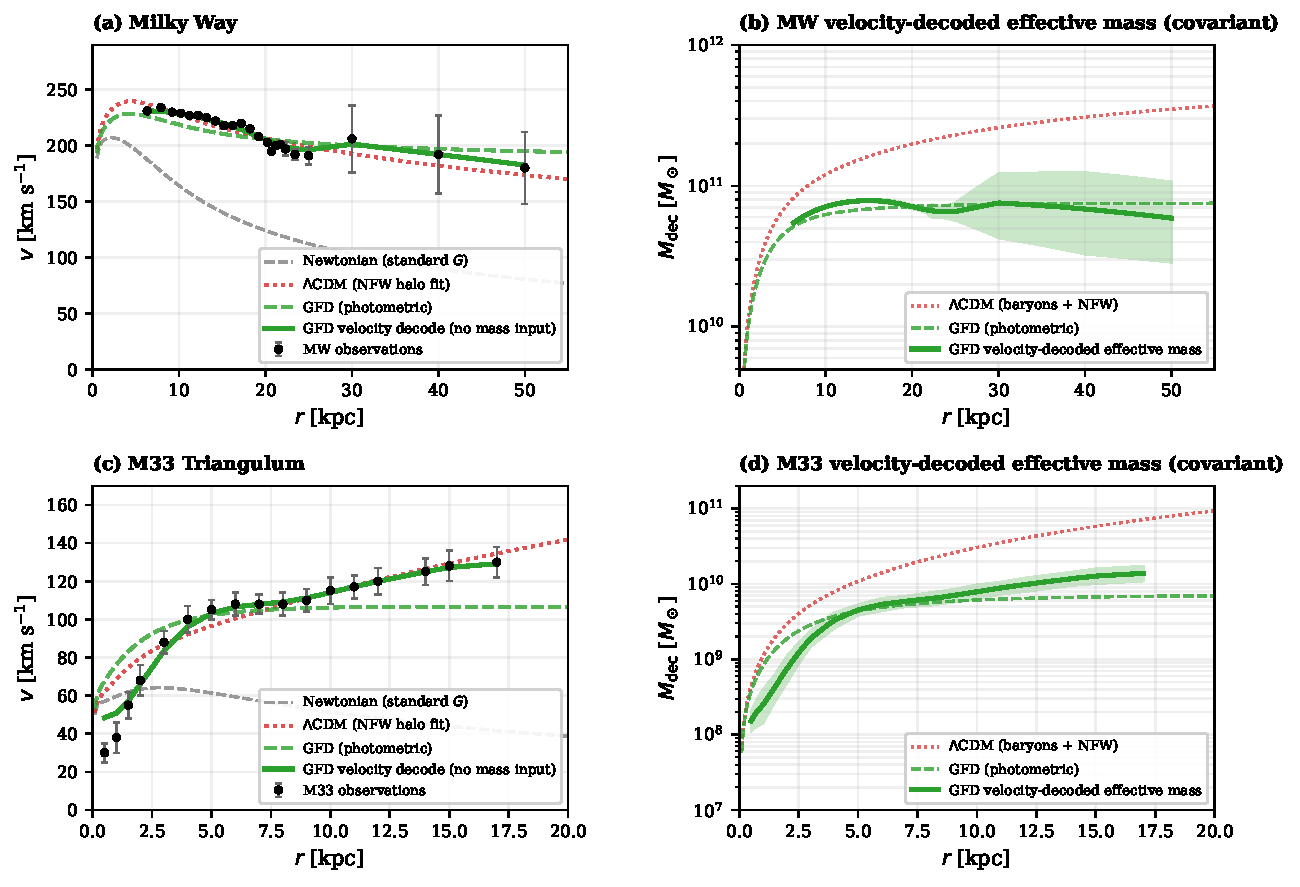
\includegraphics[width=0.98\textwidth]{fig1_mw_m33}
\caption{\textbf{Four-panel comparison for the Milky Way and M33.}
(a) Milky Way rotation curve. Observations (black) are shown with Newtonian baryons (grey dashed), $\Lambda$CDM with NFW halo (red dotted), GFD from photometric mass (green dashed), and the velocity-decoded effective mass (green solid, from observed $v$ only).
(b) Enclosed mass for the Milky Way: $\Lambda$CDM baryons+NFW (red dotted), GFD photometric (green dashed), velocity-decoded effective mass (green solid).
(c) M33 rotation curve; curve convention as in (a).
(d) M33 enclosed mass; same convention as (b).}
\label{fig:1}
\end{figure*}

% ----------------------------------------------------------------------------
% 4. DISCUSSION
% ----------------------------------------------------------------------------
\section{Discussion}
\label{sec:discussion}

We summarize what is new and what is testable. In this Letter we apply the equations in the spherically symmetric case to the Milky Way, M33, and CamB; extension to larger catalogs is outlined below.

Two things distinguish this framework. First, the constitutive law $\mu(x) = x/(1+x)$ is uniquely fixed by the field-closure postulates (Supplemental Material, Sec.~I), not selected from a family of interpolating functions. Second, the framework is built around algebraic invertibility as a zero-parameter diagnostic: from $v(r)$ alone one obtains $M_{\mathrm{dec}}(r)$ with no assumed baryonic mass distribution, no mass-to-light ratio, and no halo parameters. The inverse pipeline, velocity to mass, is the primary empirical content of this Letter.

For the Milky Way and M33, the effective mass (decoded from velocity) is consistent with baryonic mass within a factor of order unity. The framework does not require this to hold in general: photometric observations measure baryonic mass in the exterior region alone, whereas the velocity decode recovers the effective mass (the total gravitational field strength as seen by an exterior observer), which, in a spacetime with nontrivial topology, can include contributions from the throat interior. The decoded mass may therefore fall above or below the photometric value; Sec.~\ref{sec:deficit} defines the resulting deficit operationally and interprets it within the framework.

The inverse pipeline is a closed-form, mass-independent kinematic inversion: given a rotation curve and the two constants, one obtains the effective mass $M_{\mathrm{dec}}(r)$ with no halo or luminosity-to-mass assumption. Applying this pipeline to a large rotation-curve catalog such as SPARC \citep{Lelli16} (175 disk galaxies with uniform photometry and measured rotation curves) would yield effective mass profiles in one pass; systematic comparison with baryonic mass across the sample would map where the two agree and where the effective mass exceeds the baryonic contribution, providing a broad, falsifiable test of the transition and of the effective gravitational field strength that the spacetime topology sustains.

\begin{figure*}[t]
\centering
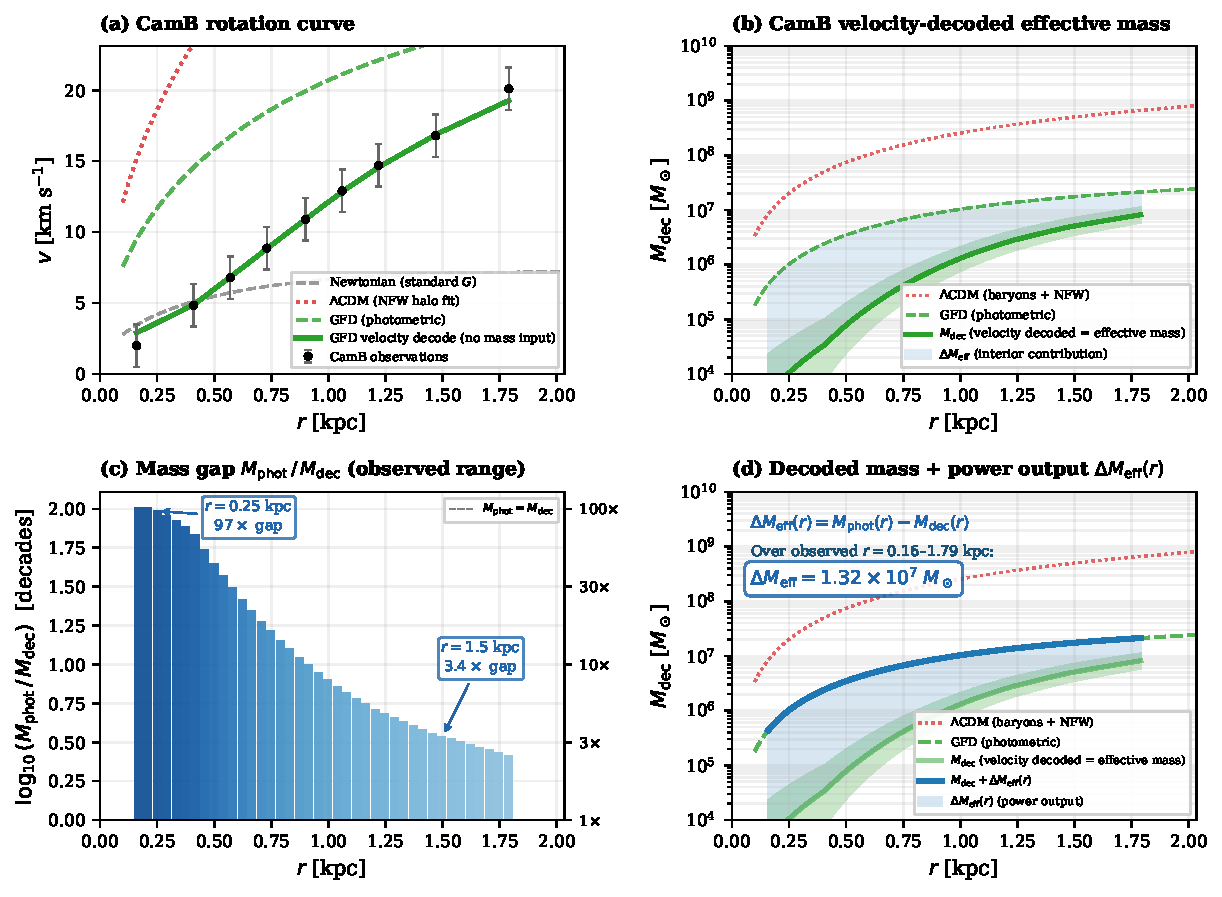
\includegraphics[width=0.98\textwidth]{fig2_camb}
\caption{\textbf{CamB: exterior vs effective mass.} (a) Rotation curve. Observations (black) with Newtonian (grey dashed), $\Lambda$CDM with NFW (red dotted), GFD photometric (green dashed), and velocity decode (green solid). (b) Enclosed mass: $\Lambda$CDM (red dotted), GFD photometric (green dashed), velocity-decoded effective mass (green solid); shaded region is $\Delta M_{\mathrm{eff}}$. (c) Mass ratio $M_{\mathrm{phot}}/M_{\mathrm{dec}}$ over the observed range. (d) Decoded mass plus $\Delta M_{\mathrm{eff}}(r)$ (blue) matches photometric (green dashed); shaded region is the interior contribution to the observed field.}
\label{fig:camb}
\end{figure*}

\subsection{Where photometric and decoded mass differ}
\label{sec:deficit}

In some galaxies the effective mass (decoded from velocity) falls below the photometric baryonic mass; the pipeline still yields a well-defined decoded profile, but the effective mass no longer matches the baryons to within a factor of order unity. This is expected rather than anomalous.

In general relativity, spacetimes with nontrivial topology (such as Ellis drainhole solutions \citep{Ellis73} or Einstein-Rosen bridges \citep{Einstein35}, structures whose astrophysical counterparts reside at the centers of spiral galaxies) permit an exterior gravitational field that is not uniquely determined by the exterior matter distribution. The interior geometry can sustain or modify the field that governs the rotation; baryons in the exterior trace the resulting dynamics but do not uniquely set their strength. A mismatch between the tracer-inferred mass and the effective field strength is therefore generic to systems whose topology includes an interior that contributes to the observed dynamics.

Because the covariant inverse pipeline decodes the effective mass from observed velocity with no mass model, the difference between photometric and velocity-decoded mass is well defined at each radius; a researcher can quantify it directly from velocity observations and the inverse pipeline, with no additional parameters. The mass deficit $\Delta M_{\mathrm{eff}}(r) = M_{\mathrm{phot}}(r) - M_{\mathrm{dec}}(r)$, with $M_{\mathrm{dec}}$ from Eq.~\ref{eq:Mdec}, measures the difference between exterior baryonic mass and the effective mass inferred from the field: the additional field strength sustained by the interior topology. Crucially, $\Delta M_{\mathrm{eff}}(r)$ is not a fitted mass model but a zero-parameter output from kinematics; it quantifies the gravitational power output sustained by the interior topology rather than invoking invisible matter. Figure~\ref{fig:camb} illustrates this for the low-surface-brightness galaxy CamB: the velocity decode matches the rotation curve, and the mass panels show the gap and its interpretation as power output from the topology. We do not resolve the interior dynamics here; the framework defines this quantity operationally. Systematic study across a range of morphologies and field strengths could map how the topological contribution varies with galactic structure and environment. The relationship is analogous to a fluid vortex: tracers follow the flow but do not determine the power output of the drain beneath.

% ----------------------------------------------------------------------------
% 5. CONCLUSIONS (start on page 4, continue page 5 left; Fig.~3 on page 5 right)
% ----------------------------------------------------------------------------
\section{Conclusions}
\label{sec:conclusions}

A central result of this letter is a closed-form expression for the effective mass. From an observed rotation curve $v(r)$, Eq.~\ref{eq:Mdec} gives
\begin{equation*}
M_{\mathrm{dec}}(r) = \frac{r\,v^4}{G\,(a_0\,r + v^2)}
\end{equation*}
with no iteration, no mass model, and no dark matter halo. We demonstrated this on the Milky Way and M33 (Fig.~\ref{fig:1}), where the decoded effective mass is consistent with known baryons within a factor of about two while $\Lambda$CDM requires several times more mass in halos to match the same velocities.

To test the framework further, we turn to NGC~3198, the canonical rotation-curve case in dark matter studies, with well-measured HI kinematics and independently inferred baryonic mass. As Fig.~\ref{fig:ngc3198} shows, the same equation, $G$, and $a_0$ yield a velocity-decoded effective mass (solid green) that tracks the known baryonic content and stays well below the $\Lambda$CDM enclosed mass (red dotted). No gravitational parameters are fitted: one formula, zero free parameters. Where the decoded effective mass falls below the photometric value, as in CamB (Fig.~\ref{fig:camb}), the deficit is equally well defined and measures the contribution that the topology sustains.

\begin{figure}[t]
\centering
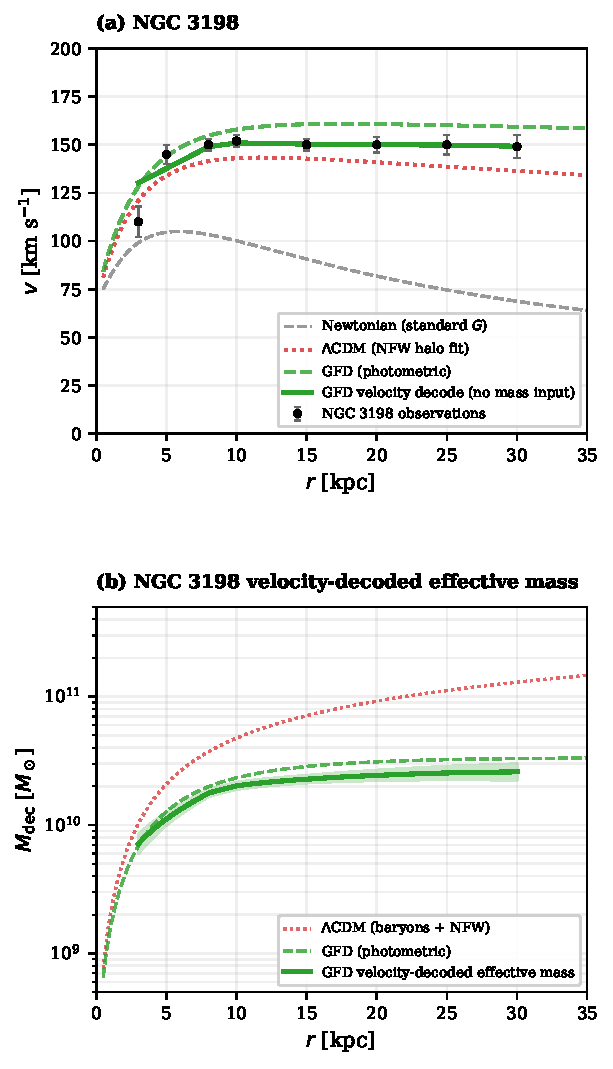
\includegraphics[width=0.88\linewidth]{fig3_ngc3198}
\caption{\textbf{NGC~3198.} (a) Rotation curve. Observations (black) with Newtonian (grey dashed), $\Lambda$CDM with NFW (red dotted), GFD photometric (green dashed), and velocity-decoded effective mass (green solid, from observed $v$ only). (b) Enclosed mass: $\Lambda$CDM (red dotted), GFD photometric (green dashed), velocity-decoded effective mass (green solid). Same Eq.~\ref{eq:Mdec}, $G$, and $a_0$ as in Fig.~\ref{fig:1}; no fitted parameters.}
\label{fig:ngc3198}
\end{figure}

Because the velocity-to-mass inversion is algebraically exact and purely kinematic, these field equations can be falsified directly by observational data. Applying this zero-parameter pipeline to surveys such as SPARC~\citep{Lelli16} will yield effective mass profiles systematically testable against baryonic mass across hundreds of galaxies.

The physical picture is simple. A galaxy, like a water vortex draining through a throat, has both an interior and an exterior. When the interior is quiet, the effective mass matches the baryons: the visible matter accounts for the rotation. When the interior is active, it drives the field beyond what the exterior matter alone sustains. A bathtub drain, a jet engine, a magnetic stirrer: each produces the same exterior flow with a different interior mechanism and a different power input; the tracers in the exterior cannot distinguish them. Ping-pong balls in a water vortex: the balls follow the rotation, yet weighing them and measuring their speed does not always reveal the full power output of the drain beneath the surface. Postulating invisible ping-pong balls to account for the anomalous rotation misdiagnoses the system; measuring the power differential between the field and its tracers is the physically exact diagnostic. Baryons play the role of the ping-pong balls; the throat interior plays the role of the drain; and the mass deficit $\Delta M_{\mathrm{eff}}(r)$ measures the power output of the drain, not a shortfall of tracers. The inverse pipeline returns the same exact equation in both regimes: when the interior is quiet, the effective mass matches the baryons; when it is active, the mass deficit $\Delta M_{\mathrm{eff}}(r)$ quantifies the topological contribution.

\section{Data and Code Availability}
\label{sec:data}
The rotation curve data used in this letter are from the published literature: \citep{McMillan17} for the Milky Way; \citep{Corbelli00} for M33; \citep{Begeman91} for NGC~3198; \citep{Lelli16} for CamB. Code: \texttt{generate\_letter\_figures.py}, \texttt{run\_all\_validations.py}. Supplemental: \texttt{supplemental\_material.pdf}.

% ----------------------------------------------------------------------------
% REFERENCES (flow in column 1 under Data and Code)
% ----------------------------------------------------------------------------
\bibliographystyle{mnras}
\bibliography{letter}

\end{document}
